\section{Model 1: SOC Continuous-Time Dynamics}
\label{sec:model1}

To characterize the internal energy status of the battery, which is intrinsically difficult to measure directly, the State of Charge (SOC) is employed as an equivalent quantitative metric. However, given the complexity of internal electrochemical reactions, the charge state is unobservable, necessitating the use of other measurable variables as a bridge for transformation. Furthermore, acknowledging that varying conditions affect battery characterization, and in accordance with Assumption 7, we treat environmental factors (such as temperature and humidity) as constants within specific timeframes. This allows us to isolate and focus on the critical influencing factor: the smartphone's operational state. Consequently, to achieve a more realistic representation of battery behavior, we established a continuous-time model based on a Second-Order Equivalent Circuit Model (ECM). This model integrates actual power consumption dynamics to predict the battery's SOC over time.



\subsection{SOC Dynamics: Coulomb Counting}
\label{subsec:soc_dynamics}

To characterize the battery's energy status using mathematical and physical modeling, we investigated the fundamental mechanism of power consumption: the cumulative inflow and outflow of electric charge. Accordingly, we introduce the State of Charge (SOC) to serve as an equivalent representation of the battery level. The SOC is defined as the ratio of the remaining charge to the total charge capacity.
\begin{equation}
    SOC(t) = \frac{Q_{\text{remaining}}(t)}{Q_{\text{usable}}}
\end{equation}

By further developing this formulation and differentiating both sides with respect to time $t$, we obtain:

\begin{equation}
    \boxed{\frac{dSOC}{dt} = -\frac{I(t)}{Qnom \cdot SOH \cdot 3600}}
    \label{eq:soc_dynamics}
\end{equation}

Further transforming charge into current to simplify calculations:

\subsection{Second-Order Equivalent Circuit Model (2-RC ECM)}
\label{subsec:ecm}

Given the difficulty in directly measuring internal battery current and the complexity of internal electrochemical reactions, from an engineering perspective, we approximate the system using a Second-Order R-C Equivalent Circuit Model (ECM) \cite{Hu2012, Chen2006}. This approach aims to transform abstract, unobservable dynamics into a computable physical model, thereby facilitating enhanced prediction and experimentation. Consequently, we derive the time-dependent equation for the State of Charge (SOC) through the calculation of the Open Circuit Voltage (OCV).

\begin{figure}[H]
    \centering
    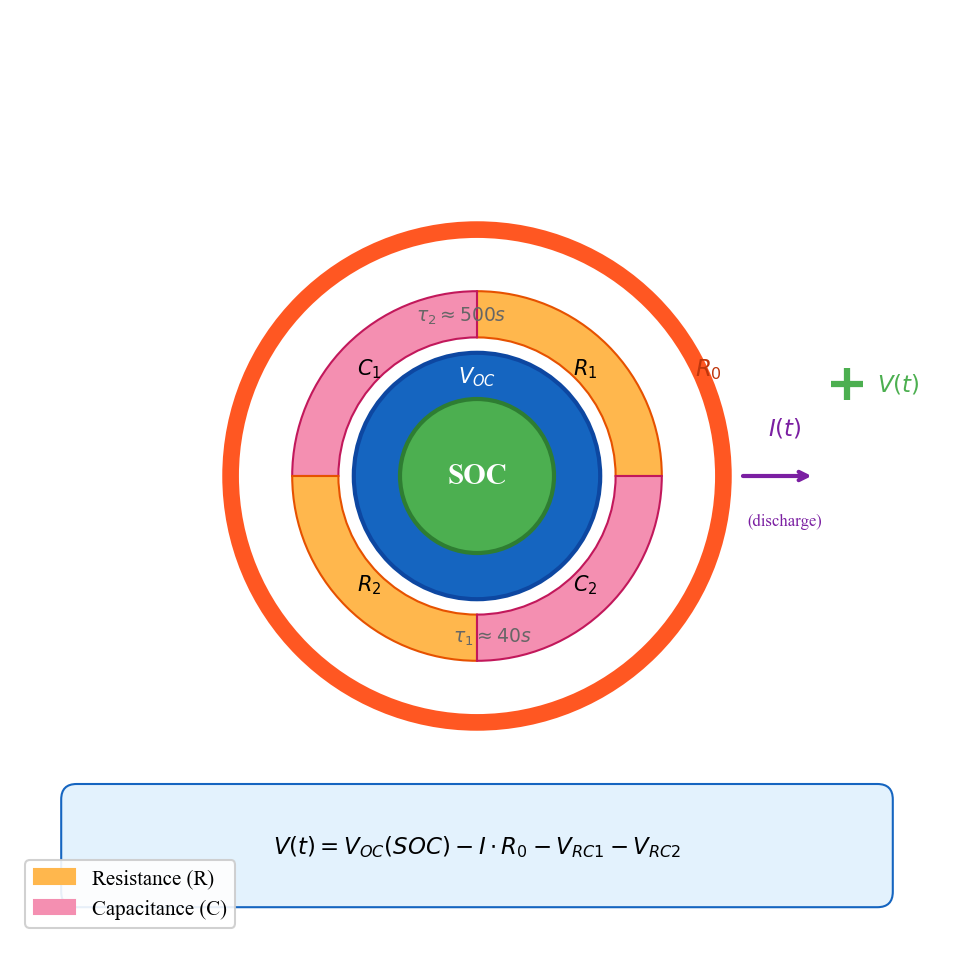
\includegraphics[width=0.75\textwidth]{figures/5F45DFA34F11539722084181119697B7.png}
    \caption{Second-order Thevenin equivalent circuit model of the battery. The model consists of an ideal voltage source $V_{OC}(\SOC)$, a series resistance $R_0$, and two RC branches with time constants $\tau_1 \approx 40$~s and $\tau_2 \approx 500$~s representing fast and slow polarization dynamics, respectively.}
    \label{fig:ecm_circuit}
\end{figure}

Based on the circuit diagram, we formulate the voltage equations for the R-C branches in accordance with fundamental physical principles:

\begin{align}
    \frac{dV_{RC1}}{dt} &= -\frac{V_{RC1}}{\tau_1(T)} + \frac{I(t)}{C_1} \label{eq:vrc1} \\
    \frac{dV_{RC2}}{dt} &= -\frac{V_{RC2}}{\tau_2(T)} + \frac{I(t)}{C_2} \label{eq:vrc2}
\end{align}

For the calculation and measurement of the Open Circuit Voltage (OCV), we adopt an approach based on electrochemical principles. Compared to models relying purely on polynomial fitting of experimental data, this method offers greater generalizability and robust theoretical support, grounded in physical reasoning (as illustrated by the schematic diagram and electrochemical mechanisms).

The underlying chemical reaction is described by:
$$ Li^+ + e^- + CoO_2 \leftrightarrow LiCoO_2 $$

Consequently, the potential is governed by the Nernst equation:
$$ E_{pos} = E^0_{pos} - \frac{RT}{F} \ln \left( \frac{[LiCoO_2]}{[CoO_2] \cdot [Li^+]} \right) $$

\hspace*{\parindent}Thus, starting from the fundamental form of the Nernst equation, we further rearrange it into a formulation suitable for lithium-ion battery mechanisms:
\begin{equation}
    E(x) = E^0 + \frac{RT}{F} \ln\left(\frac{1-x}{x}\right)
    \label{eq:nernst_simplified}
\end{equation}

\hspace*{\parindent}Since the lithium-ion concentration at the positive electrode can be approximated as proportional to the accumulated charge (and hence treated as an SOC-equivalent state), the expression can be rewritten as:
\begin{equation}
    E(\SOC) = E^0 + \frac{RT}{F} \ln\left(\frac{1-\SOC}{\SOC}\right)
    \label{eq:nernst_soc}
\end{equation}

\hspace*{\parindent}However, using the Nernst equation alone to compute the open-circuit voltage (OCV) has limitations. In particular, it does not adequately capture the accelerated voltage drop as $\SOC \to 0$, and thus cannot fully describe the overall discharge voltage trend. Therefore, we introduce the Shepherd model as an empirical refinement:
\begin{equation}
    V_{\text{batt}} = E_0 - R\, i - K \frac{Q}{Q - it}\, i + A \cdot \exp(-B\, it)
    \label{eq:shepherd}
\end{equation}

By optimizing the polarization of this model and incorporating it into the Nernst model, a more complete open-circuit voltage model can be obtained.

\begin{equation}
    \boxed{\OCV(\SOC, T) = K_0 + K_1 \cdot \SOC + K_2 \cdot \ln(\SOC) + K_3 \cdot \ln(1-\SOC) + \frac{\partial \OCV}{\partial T}(T - \Tref)}
    \label{eq:ocv}
\end{equation}

\begin{figure}[H]
    \centering
    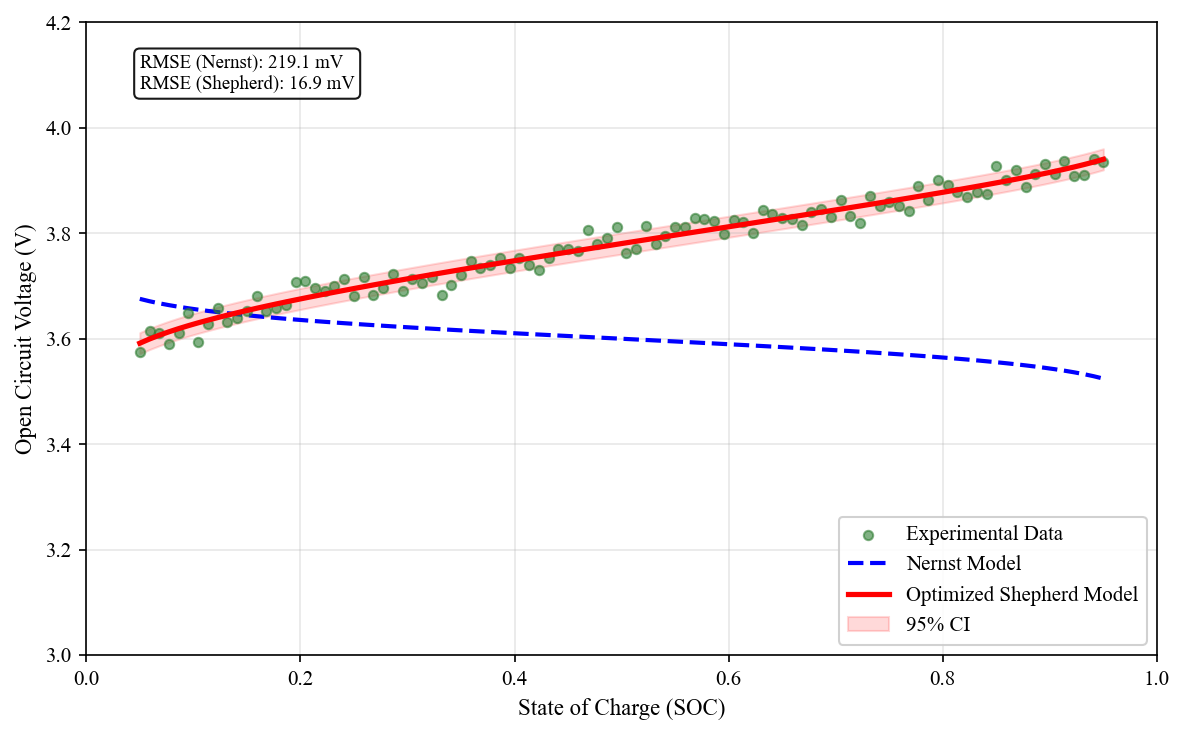
\includegraphics[width=0.8\textwidth]{figures/40949D9BDBCBDD5ACBFD6D84D3CBE06B.png}
    \caption{Comparison of OCV models versus experimental data. The optimized Shepherd model (RMSE = 16.9~mV) demonstrates significantly better fit than the basic Nernst model (RMSE = 219.1~mV), particularly capturing the characteristic voltage plateau in the mid-SOC region and the steep drop at low SOC.}
    \label{fig:ocv_fitting}
\end{figure}

\begin{figure}[H]
    \centering
    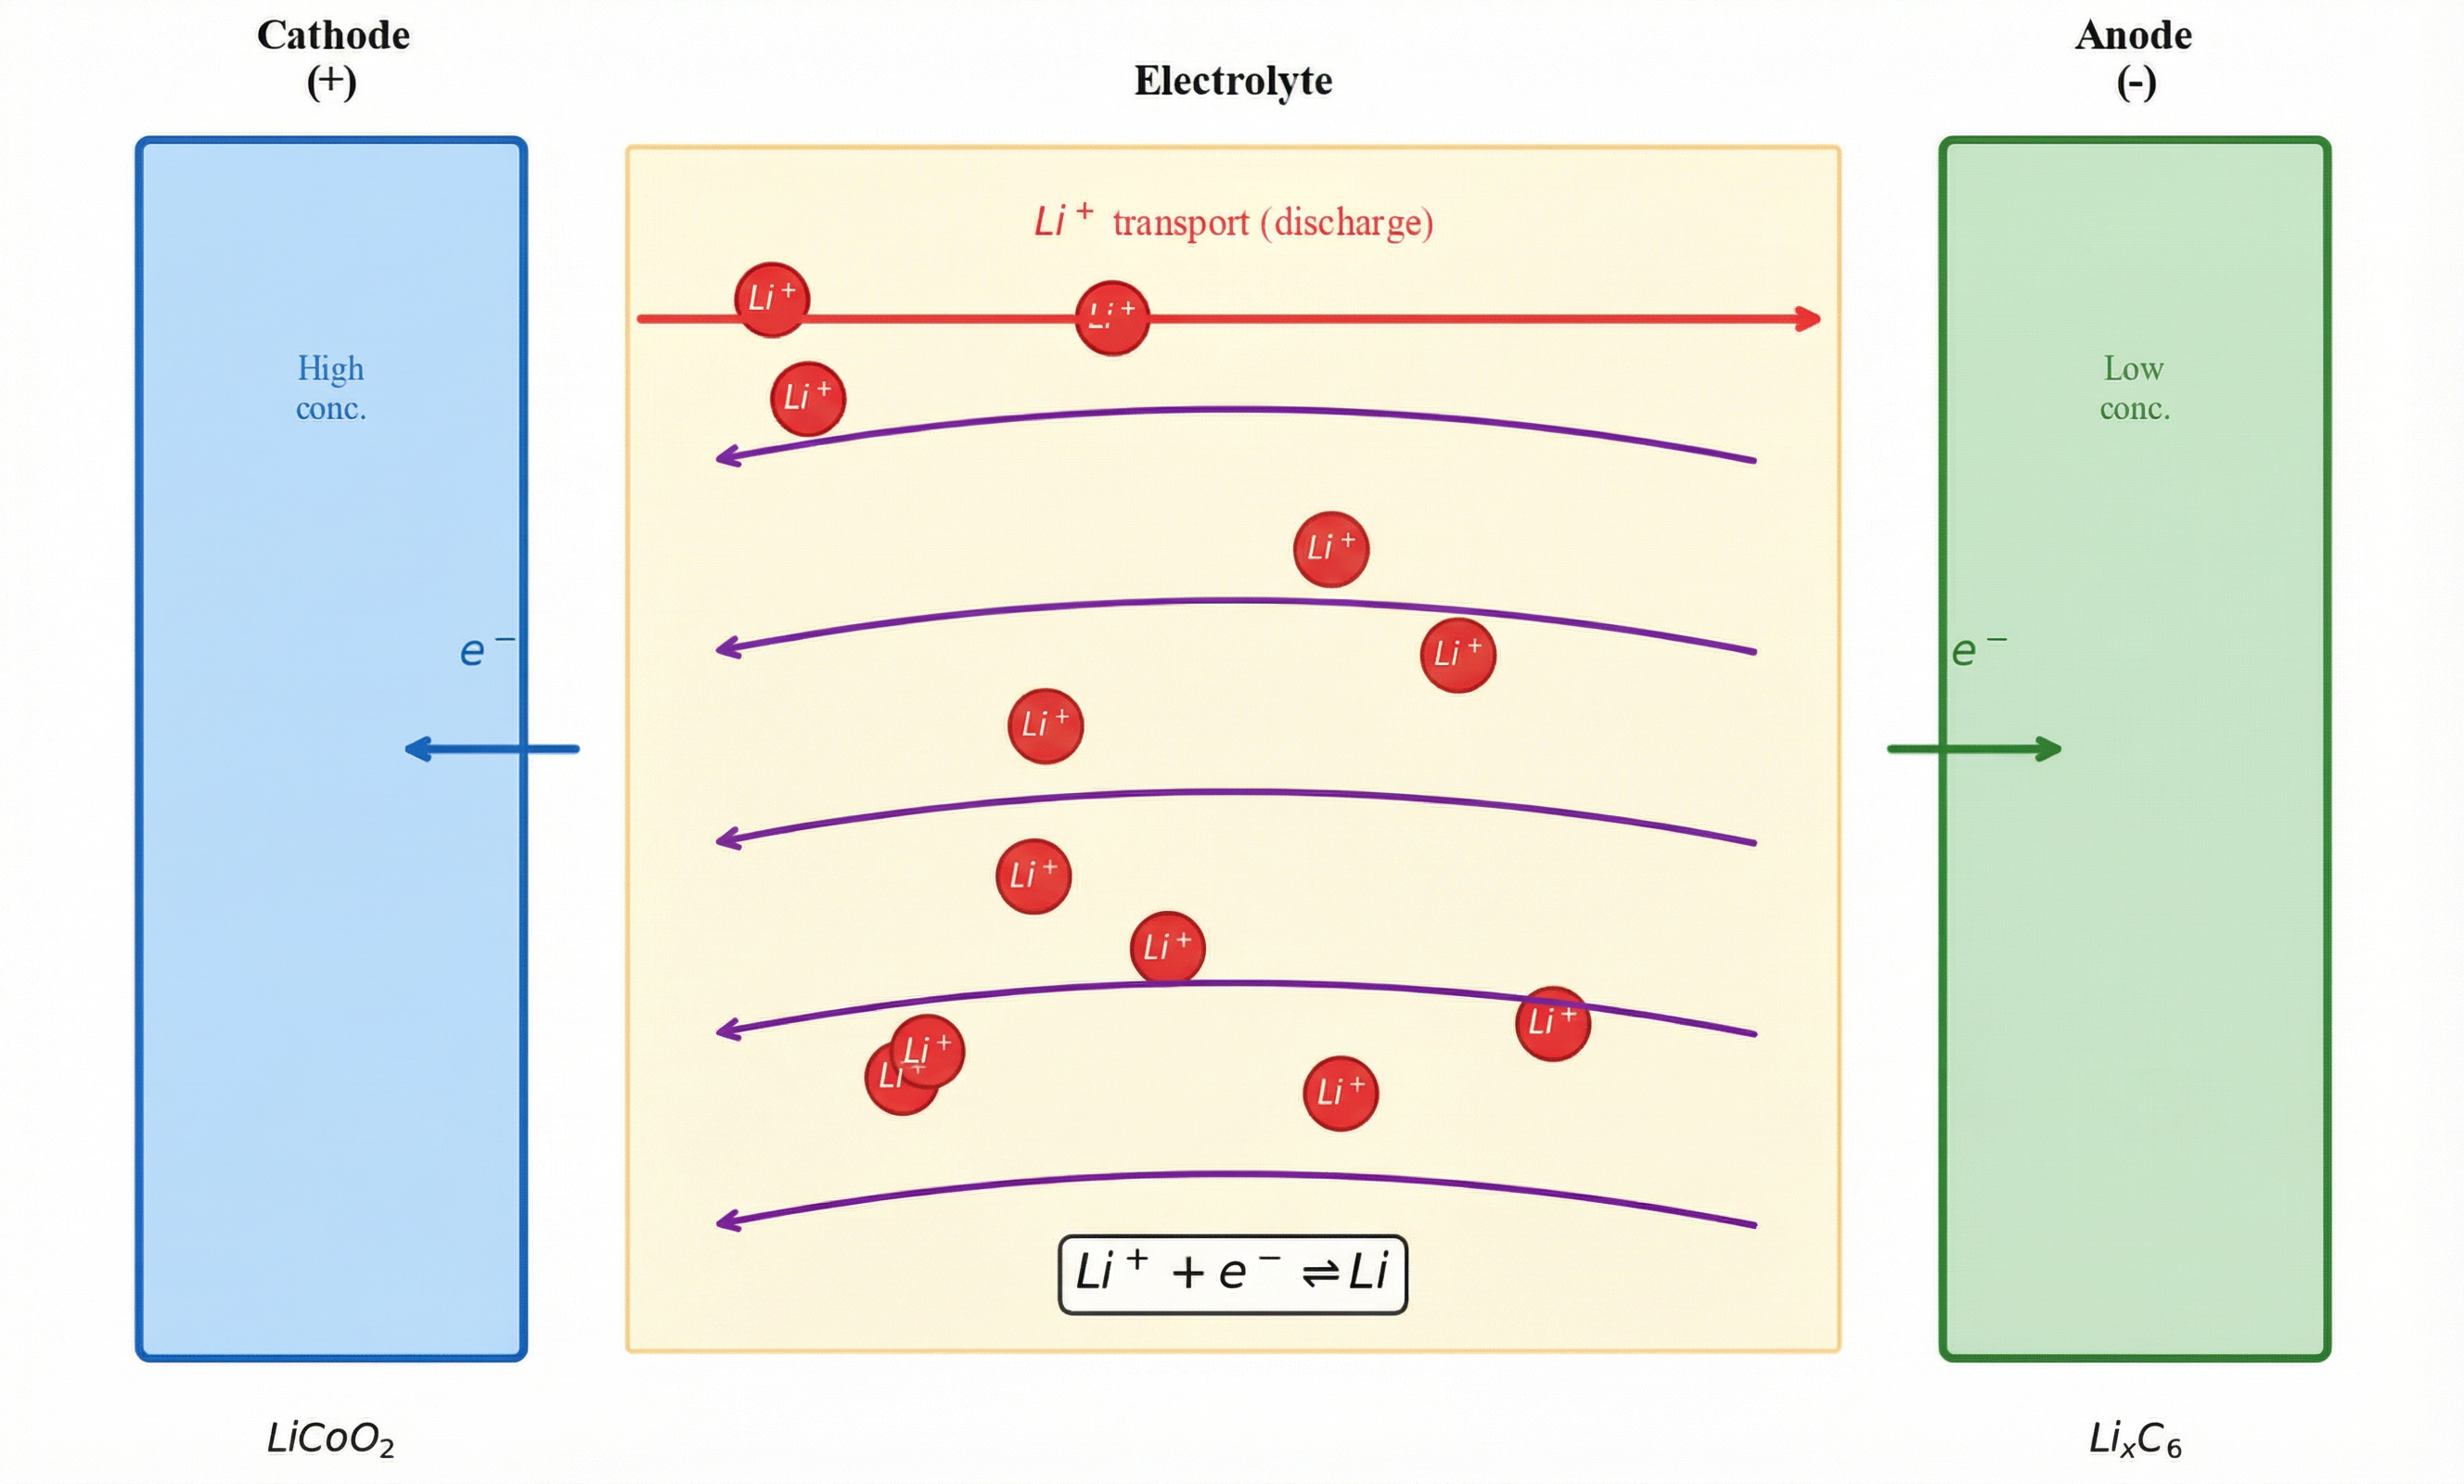
\includegraphics[width=0.8\textwidth]{figures/figure/629DA22DA5B3F71BCC7717D7D02E0C7A.png}
    \caption{Detailed OCV-SOC characterization with uncertainty bounds. The scatter plot shows experimental measurements (green dots), the basic Nernst model (blue dashed line), and the optimized Shepherd model (red solid line) with 95\% confidence band. The Shepherd model achieves significantly lower RMSE, validating its use in the continuous-time SOC dynamics model.}
    \label{fig:ocv_fitting_detailed}
\end{figure}

Finally, by combining the above models, a more accurate continuous-time model of SOC (a system of differential equations) can be obtained. The thermal equation follows the lumped-parameter approach \cite{Bernardi1985, Pesaran2002}.

\begin{equation}
    \boxed{
    \begin{aligned}
        \frac{d\SOC}{dt} &= -\frac{I(t)}{\Qnom \cdot \SOH \cdot 3600} \\[6pt]
        \frac{dV_{RC1}}{dt} &= -\frac{V_{RC1}}{\tau_1(T)} + \frac{I(t)}{C_1} \\[6pt]
        \frac{dV_{RC2}}{dt} &= -\frac{V_{RC2}}{\tau_2(T)} + \frac{I(t)}{C_2} \\[6pt]
        \frac{dT}{dt} &= \frac{I^2 R(T,\SOC) - h_{\text{eff}}A(T-\Tamb)}{mC_p} \\[6pt]
        \frac{d\SOH}{dt} &= -\dot{\SOH}_{\text{cal}}(T, \SOC) - \dot{\SOH}_{\text{cyc}}(I, T, \SOC)
    \end{aligned}
    }
    \label{eq:full_ode}
\end{equation}

with state vector $\mathbf{x} = [\SOC, V_{RC1}, V_{RC2}]^T$.

\subsection{Power-to-Current Conversion}
\label{subsec:power_current}

\hspace*{\parindent}In practical use, smartphones operate in different working states, each associated with a distinct power consumption profile, which leads to different SOC trajectories. Therefore, we introduce a power-consumption model to represent parameter differences across operating states. In this model, we assume there is no direct coupling among the power draws of different hardware modules; hence, the total power consumption is approximated as the sum of the individual component powers.

\begin{equation}
    P_{\text{total}}(t) = P_{\text{display}} + P_{\text{CPU}} + P_{\text{network}} + P_{\text{GPS}} + P_{\text{base}} + P_{\text{other}}
    \label{eq:power_total}
\end{equation}

\begin{figure}[H]
    \centering
    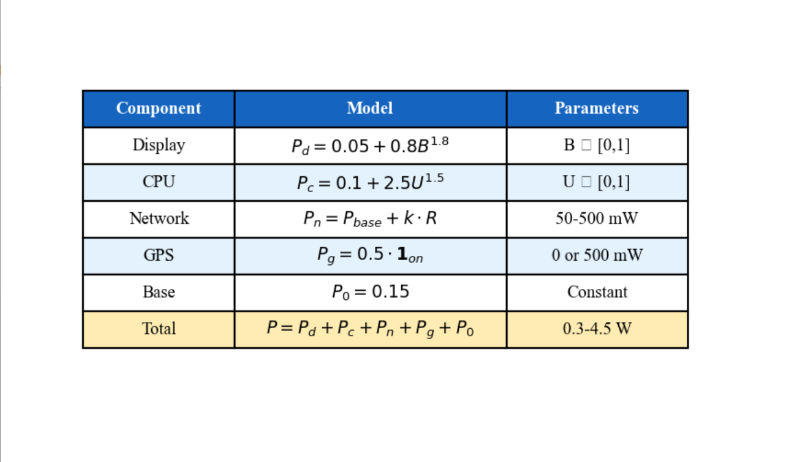
\includegraphics[width=0.7\textwidth]{figures/B05BE26D1ADE5254D2A58C0F9CCE878C.png}
    \caption{Power consumption component models and parameters for smartphone hardware. Each component follows a specific power model based on utilization, with display and CPU being the dominant contributors.}
    \label{fig:power_model_table}
\end{figure}

\begin{figure}[H]
    \centering
    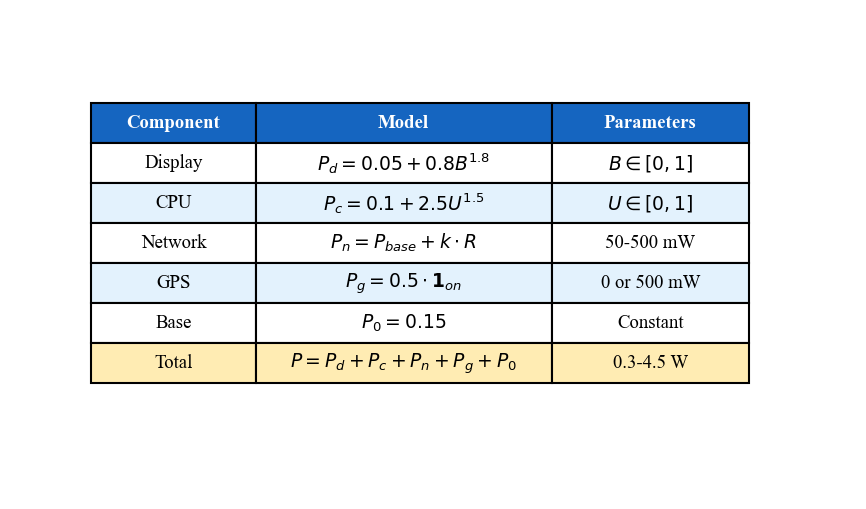
\includegraphics[width=0.75\textwidth]{figures/figure/430B0656941AF15F8DE95C64258776AE.png}
    \caption{Detailed power consumption model parameters. The table summarizes mathematical expressions for each component: Display power follows $P_d = 0.05 + 0.8B^{1.8}$ with brightness $B \in [0,1]$; CPU power follows $P_c = 0.1 + 2.5U^{1.5}$ with utilization $U \in [0,1]$; Network power ranges from 50--500~mW; GPS consumes 500~mW when active; and the baseline power is 150~mW.}
    \label{fig:power_model_detailed}
\end{figure}

\begin{figure}[H]
    \centering
    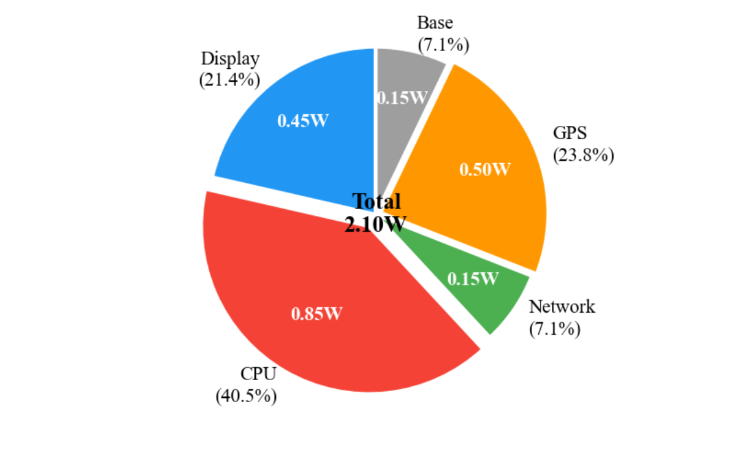
\includegraphics[width=0.55\textwidth]{figures/DE80970C2134029C2340572AAFAE6797.png}
    \caption{Power consumption breakdown under typical usage scenario (total 2.10~W). The CPU accounts for the largest share (40.5\%), followed by GPS (23.8\%) and display (21.4\%).}
    \label{fig:power_breakdown}
\end{figure}

\begin{figure}[H]
    \centering
    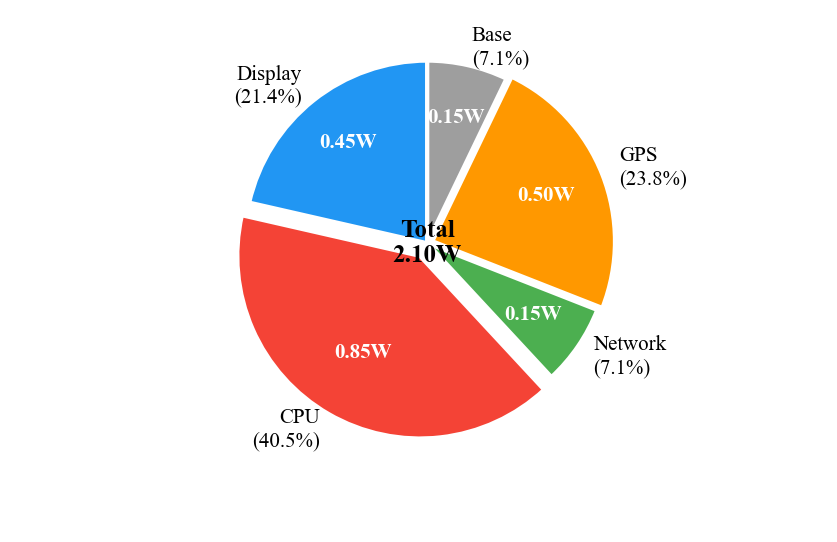
\includegraphics[width=0.55\textwidth]{figures/figure/AD0B64CF52E17EDAD0FCFF43D8E14684.png}
    \caption{Alternative power consumption breakdown visualization showing the same distribution: CPU (0.85~W, 40.5\%), GPS (0.50~W, 23.8\%), Display (0.45~W, 21.4\%), Network (0.15~W, 7.1\%), and Base (0.15~W, 7.1\%), totaling 2.10~W.}
    \label{fig:power_breakdown_alt}
\end{figure}

At this point, the difficult-to-measure current can be converted into a power-to-voltage ratio.

\begin{equation}
    I(t) = \frac{P(t)}{V(t)}
\end{equation}

The current calculation can be considered as solving the basic KVL equation in the algebraic loop of a second-order RC circuit.


\begin{equation}
    I = \frac{(OCV - V_{RC1} - V_{RC2}) - \sqrt{(\OCV - V_{RC1} - V_{RC2})^2 - 4R_0 P}}{2R_0}
    \label{eq:current_solve}
\end{equation}


Substituting the obtained expressions for current and terminal voltage into the continuous-time differential equations, we obtain the optimized model for the overall power.